\documentclass[a4paper,twoside,12pt]{article}
\usepackage[T1]{fontenc}
\usepackage[utf8]{inputenc}
\usepackage[english]{babel}
%\usepackage[english=nohyphenation]{hyphsubst} % Tällä englannin tavutus pois.
%\usepackage[sc]{mathpazo} % Vaihtoehtoinen Palatino-fontti käyttöön.
\usepackage{enumerate}
\usepackage[shortlabels]{enumitem}
\usepackage{fullpage}
\usepackage{setspace}
\usepackage{graphicx}
\usepackage{import}
\usepackage{amsmath}
\usepackage{mathabx}
\usepackage{icomma}
\usepackage{booktabs}
\usepackage{ftcap}
\usepackage{lipsum}
\usepackage{url}
\usepackage{siunitx}
\usepackage{epstopdf}
\usepackage{hyperref}

\begin{document}
\onehalfspacing%  % Riviväli 1.5.
\thispagestyle{empty}
\begin{flushleft}
 \underline{Sakari} Matias Kapanen\hfill
 \texttt{sakari.m.kapanen@student.jyu.fi}
\end{flushleft}
\vfill
\begin{center}
\textsc{\LARGE FYSS430 A computer tomographic study of the infill ratio of a 3D printed object}
\end{center}
\vfill
Measurement date: January 25, 2017\\
Supervisor: Arttu Miettinen\\
\vfill
\begin{abstract}
 \noindent
    TODO
\end{abstract}
\clearpage%

\setlength{\parindent}{0pt}  % Kappaleen alkuun ei sisennystä.
\setlength{\parskip}{12pt}  % Sen sijaan kappaleiden väliin rako.

\setcounter{page}{1}

\section{Introduction}
Three-dimensional printing is an additive manufacturing method where plastic is extruded layer by layer to produce a three-dimensional object. A solid 3D CAD model is prepared for printing by a ``slicer'' software which generates the tool paths for the nozzle.

It does not often make sense to fill the whole solid model with plastic. Therefore a sparse ``infill'' pattern is generated instead as shown in image~\ref{fig:honeycomb}.

The volumetric ratio of the infill material inside the cube was chosen as the research subject of this computer tomography project work. Tomographic imaging makes it possible to acquire a volume image of the 3D printed cube which can be then analyzed by traditional image analysis methods.

\begin{figure}
    \centering
    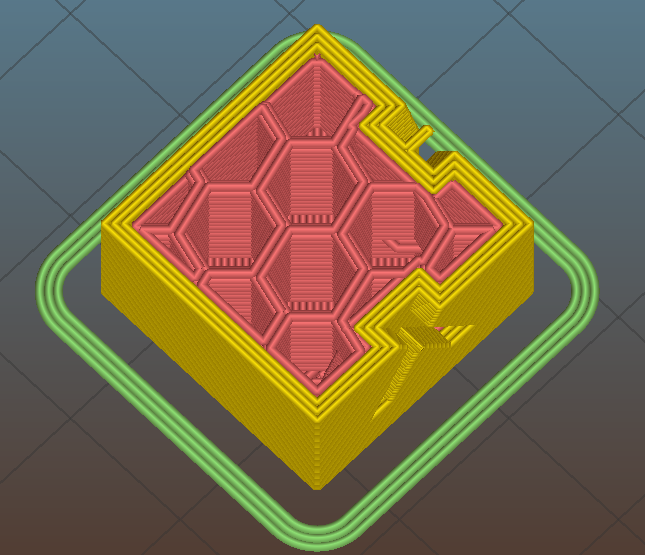
\includegraphics[width=0.8\textwidth]{images/cube_slic3r.png}
    \caption{A section of a three-dimensional cube model~\cite{testcube} sliced by Slic3r~\cite{slic3r}. A honeycomb infill pattern of 20 \% ratio has been generated inside.}
    \label{fig:honeycomb}
\end{figure}

\section{Theoretical background}
\subsection{X-ray computer tomography and reconstruction}

\subsection{Image analysis}

\section{Experimental methods}
\subsection{SkyScan 1172 CT scanner}

\subsection{Image analysis software}

\section{Results}

\section{Conclusions}

\clearpage

\begin{thebibliography}{9}
    \selectlanguage{english}
    \bibitem{testcube} XYZ 20mm Calibration Cube. iDig3Dprinting. \url{http://www.thingiverse.com/thing:1278865/#files}. Referenced March 7, 2017.
    \bibitem{slic3r} Slic3r, G-code generator for 3D printers. \url{http://slic3r.org/}. Referenced March 7, 2017.
\end{thebibliography}

\end{document}

